\subsection{Scalar field in dS space-time}\label{sec:dS}
Use conformal time in the metric. Cosnider a real, minimally coupled scalar field $\phi(x^\mu)$:
\begin{eqopt}
    S=\frac{1}{2}\int d^4x \sqrt{-g} \left( \partial_\mu \phi \partial^\mu \phi -  m^2 \phi^2 \right)
\end{eqopt}
Rescale with \textcolor{darkgreen}{$\chi \equiv a \phi$} and eventually define \textcolor{darkgreen}{$m_{\text{eff}}^2 \equiv m^2a^2-\frac{a^{\prime\prime}}{a}$}
Action is explicitly time dependent $\Rightarrow$ energy not conserved $\Rightarrow$  particle creation (with energy supplied by the classical gravitational field).
Get EOM for $\chi$, then expand in Fourier modes:
\begin{eqopt}
    \chi(\mathbf{x},\tau) = \int \frac{d^3k}{(2\pi)^{3/2}} \chi_{\mathbf{k}}(\tau) e^{i\mathbf{k}\cdot\mathbf{x}} \label{Fourier}
\end{eqopt}
Rewrite EOM in terms of $\chi_{\mathbf{k}}$. Note that $\chi$ is a real number $\Rightarrow \chi_{\mathbf{k}}^* = \chi_{-\mathbf{k}}$. EOM just depends on $\abs{\mathbf{k}}$, general solution is
\begin{eqopt}[darkred]\label{Mode_exp}
    \chi_{\mathbf{k}}(\tau) = \frac{1}{\sqrt{2}} \left( a^-_{\mathbf{k}} \, v^*_k(\tau) + a^+_{-\mathbf{k}}\, v_k(\tau)  \right) 
\end{eqopt}
\emph{$a_{\mathbf{k}}$ coefficients are not yet identified as annihilation/creation operators, $v_k$ are called mode functions.} Normalization is \textcolor{darkred}{$\Im(v^{\prime}v^*)=1/2$}. 
Put back in~\eqref{Fourier}
\begin{equation}\label{Fourier_v}
\chi(\mathbf{x}, \tau) = \frac{1}{\sqrt{2}} \int \frac{d^3 k}{(2\pi)^{3/2}} \left[ a^-_{\mathbf{k}} v_k^*(\tau) e^{i \mathbf{k} \cdot \mathbf{x}} + a_{-\mathbf{k}}^+ v_k(\tau) e^{-i \mathbf{k} \cdot \mathbf{x}} \right]
\end{equation}
EOM for $v_k$ is
\begin{equation}
    v_k^{\prime\prime} + \overbrace{\left( k^2 + m_{\text{eff}^2} \right)}^{\omega_k^2} v_k = 0
\end{equation}

Define canonical momentum and Hamiltonian:
\begin{eqopt}[darkgreen]
\Pi = \frac{\partial \mathcal{L}}{\partial \chi'} \qquad \hat{\mathcal{H}} = -\mathcal{L} + \hat{\Pi} \chi' \color{black} = \frac{1}{2}\int d^3x \left( \hat{\Pi}^2 + \left(\nabla \hat{\chi}\right)^2 + m_{\text{eff}}^2 \hat{\chi}^2 \right)
\end{eqopt}
Impose equal time commutation relations: $[\hat{\chi}(x, \tau), \hat{\Pi}(y, \tau)] = i \delta^3(x - y)$

Here one may show that, promoting the coefficients $a_{\mathbf{k}}$ to operators, they obey commutation relations of annihilation/creation operators; with which one can construct quantum states of the theory.
\begin{equation}
    \ket{m_{\mathbf{k_1}}, n_{\mathbf{k_2}}, \ldots} = \frac{1}{\sqrt{m!n!\ldots}}(\hat{a}_{\mathbf{k}_1}^\dagger)^m(\hat{a}_{\mathbf{k}_2}^\dagger)^n\ldots \ket{0}
\end{equation}

%Bogoliubov transformation
\begin{mycolorbox}[red!50!orange]
    \textbf{Bogoliubov transformation:}

\begin{eqopt}
    u_k(\tau) = \alpha_k v_k(\tau) + \beta_k v^*_k(\tau)
\end{eqopt}
Impose normalization condition on $u_k$: $u_k^{\prime}u_k^* - u_k^{\prime *}u_k=i$ to get \textcolor{darkred}{$\abs{\alpha_k}^2 - \abs{\beta_k}^2 = 1$}.
\begin{equation}\label{Fourier_u}
    \chi(\mathbf{x}, \tau) = \frac{1}{\sqrt{2}} \int \frac{d^3 k}{(2\pi)^{3/2}} \left[ b^-_{\mathbf{k}} u_k^*(\tau) e^{i \mathbf{k} \cdot \mathbf{x}} + b_{-\mathbf{k}}^+ u_k(\tau) e^{-i \mathbf{k} \cdot \mathbf{x}} \right]
    \end{equation}
To find relation between $b_{\mathbf{k}}$ and $a_{\mathbf{k}}$, equate~\eqref{Fourier_v} and~\eqref{Fourier_u}
A generic state is 
\begin{equation}
    \ket{\psi} = \sum_{m,n,\ldots} C_{mn\dots}^A \ket{m_{\mathbf{k_1}}, n_{\mathbf{k_2}}, \ldots}_A = \sum_{m,n,\ldots} C_{mn\dots}^B \ket{m_{\mathbf{k_1}}, n_{\mathbf{k_2}}, \ldots}_B
\end{equation}
with $\ket{m_{\mathbf{k_1}}, n_{\mathbf{k_2}}, \ldots}_A \equiv (m!n!\dots)^{-1/2}\ket{(\hat{a}_{\mathbf{k_1}}^\dagger)^m (\hat{a}_{\mathbf{k_2}}^\dagger)^n \dots}$

Show that \textcolor{red}{$\tensor[_B]{\langle0|}{}\,\hat N^A_{\mathbf k}\,\ket{0}_{B} = \abs{\beta_{\mathbf{k}}}^2 \delta^{(3)}(0)$}, divergence is due to infinite spatial volume.
\end{mycolorbox}

%Flat quantization
\begin{mycolorbox}[green!50!black]
    \textbf{Flat background:}
    
\emph{Hamiltonian is time independent. The vacuum is the eigenstate of the $\hat{H}$ with lowest energy.}
Substitute~\eqref{Mode_exp} in $\hat{H}$ (here $a=1 \Rightarrow m_{\text{eff}}=m$, set it to zero for convenience, since we are only interested in the fact that it is not time dependent) and define 
\begin{eqopt}[darkgreen]
    F_k \equiv v_k^{\prime 2} +k^2 v_k^2 \qquad E_k \equiv  \abs{v_k^{\prime}}^2 +k^2 \abs{v_k}^2
\end{eqopt}
Write the mode functions as $v_k = r_k(\tau) e^{i\alpha_k(\tau)}$. 
For $\ket{0}_v$ to be vacuum, $\tensor*[_v]{\expval{0|\hat{H}|0}}{_v} = \tfrac{\delta(0)}{2}\int d^3k E_k$ must be minimized.
Impose normalization condition on $v_k$ to rewrite $E_k$ and then minimize it: $dE_K/dr^\prime = 0$, $dE_K/dr = 0 $. Find mode functions that minimize energy:
\begin{equation}\label{eq:flat_vk}
    v_k = \frac{1}{\sqrt{2k}} e^{ik\tau}
\end{equation}
\end{mycolorbox} 

%dS quantization
\begin{mycolorbox}[green!50!orange]
\textbf{dS background:} \hfill $\rho=T^{00}=\Lambda/8\pi G=-T^{ii}=-P \Rightarrow H^2 = \text{const}$

\vspace{1mm}
Let \textcolor{mypurple}{$k^2\rightarrow \omega^2_k(\tau)=k^2+m_{\text{eff}}^2(\tau)$} 
\begin{equation}
    v_k(\tau_0) = \frac{1}{\sqrt{2\omega_k(\tau_0)}} e^{i\omega_k(\tau_0)\tau_0} 
\end{equation}
\emph{To these one can associate a vacuum state $\ket{0}_{\tau_0}$, which is the eigenstate of the annihilation operator $\hat{a}_{\mathbf{k}}$ at time $\tau_0$. It will not be the 
lowest energy state at later times $\rightarrow$ time dependence of the effective mass gives rise to particle creation.}

In $dS$ spacetime $a\propto e^{Ht} \; \Rightarrow\; \tau = \int_{-\infty}^t dt e^{-Ht}\; \Rightarrow\;  \tau  = -1/aH \; \Rightarrow\;  \tau \in \ointerval[scaled]{-\infty}{0} \; \Rightarrow \; m_{\text{eff}}=(aH)^2\left[(m/H)^2-2\right]$
EOM for $v_k$ becomes 
\begin{equation}\label{eq:EOMvk}
    v_k^{\prime\prime} + \Biggl[ k^2 - \frac{1}{\tau^2}\overbrace{\left(2-\frac{m^2}{H^2}\right)}^{\nu^2-1/4} \;\Biggr] v_k = 0
\end{equation}
Solution is in terms of Hankel functions:
\begin{eqopt}[darkred]
    v_k(\tau) = \sqrt{-\tau}\left[ C_1 H_\nu^{(1)}(-k\tau)+ C_2 H_\nu^{(2)}(-k\tau) \right]
\end{eqopt}
with \textcolor{darkgreen}{$\nu \equiv \sqrt{\frac{9}{4}-\frac{m^2}{H^2}}$}. \underline{Consider massless scalar field} $\Rightarrow \nu = 3/2$. This leads to
\begin{eqopt}[darkred]\label{mode_dS}
    v_k(\tau) = \left[ C_1\left(1-\frac{i}{k\tau}\right)+ C_2 \left(1+\frac{i}{k\tau}\right) \right]
\end{eqopt}
Now impose initial conditions at $\tau\ll 0$ to determine $C_1$ and $C_2$: \emph{ask the scalar to be in the instantaneous vacuum state at early times} $\Rightarrow$ $C_1=0$ and $C_2=1$ (due to limit forms of $H_\nu^{(1,2)}$) to recover the flat space limit~\eqref{eq:flat_vk}.
Note that, at early times, $k \gg 1/\tau$ as $k$ is a fixed mode~\footnote{A mode $k$ is associated with a wavelength \textcolor{darkred}{$\lambda = 2\pi/k$}, so when $k</>aH$, it is said to be super/sub-horizon meaning that the $\lambda$ is larger/smaller than the Hubble radius. We compare with the Hubble radius instead of the comoving particle horizon because the former is a local, instantaneous length scale over which causal processes can operate at that moment, while the latter is a cumulative distance that light could have traveled (monotonically increasing function).}.
\begin{center}
    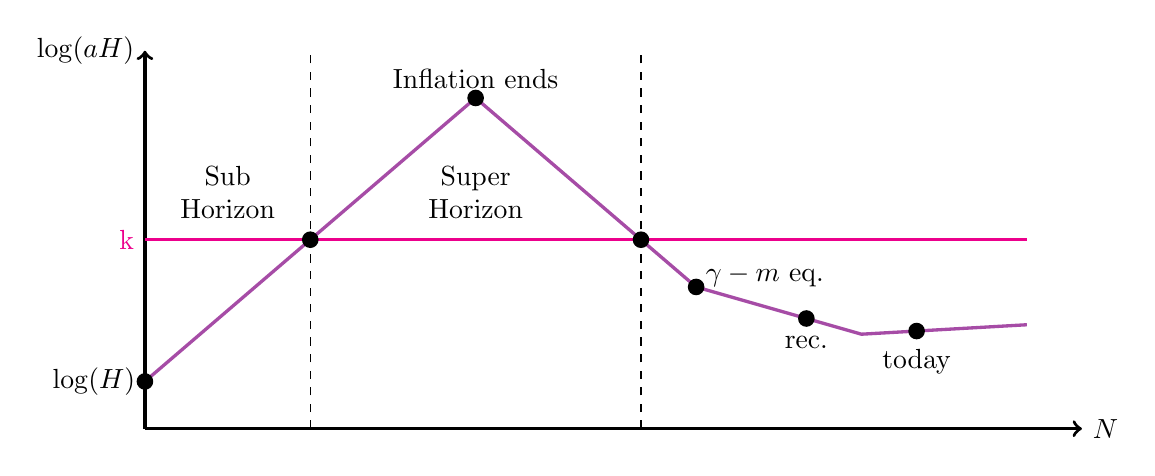
\begin{tikzpicture}[x=1.4cm,y=1.2cm]

        % --- axes -----------------------------------------------------
        \draw[very thick,->] (0,0) -- (0,4) node[below,left] {$\log(aH)$};
        \draw[very thick,->] (0,0) -- (8.5,0) node[right] {$N$};
      
        % --- horizon‐crossing “grid” (magenta) ------------------------
        \coordinate (khoriz) at (1.5,0);
        \coordinate (lhoriz) at (0,2);
      
        \draw[dashed] (khoriz) ++(0,0) -- ++(0,4);   % vertical
        \draw[dashed] (khoriz) ++(3,0) -- ++(0,4);   % vertical
        \draw[magenta,very thick]  (8,2) -- (lhoriz) node[left] {k};  % horizontal

         % --- illustrative k-mode trajectory (lavender) ----------------
         \draw[very thick,violet!70!white] 
         plot coordinates{(0,0.5) (3,3.5) (5,1.5) (6.5,1) (8,1.1)};
      
        % intersection dots 
        \fill (1.5,2) circle (3pt);
        \fill (4.5,2) circle (3pt);
        \fill (0,0.5) circle (3pt);
        \fill (3,3.5) circle (3pt) node[above] {Inflation ends};
        \fill (5,1.5) circle (3pt) node[above=4pt,right] {$\gamma-m$ eq.};
        \fill (6,1.166) circle (3pt) node[below=3pt] {rec.};
        \fill (7,1.03333) circle (3pt) node[below=3pt] {today};
      
        % --- sub-/super-horizon labels --------------------------------
        \node[align=center] at (0.75,2.5) {Sub\\Horizon};
        \node[align=center] at (3,2.5) {Super\\Horizon};

        % log(H) marker
        \draw node[left] at (0,0.5) {$\log(H)$};
      
      \end{tikzpicture}
\end{center}

The mode functions in~\eqref{mode_dS} define the \textit{\textcolor{darkgreen}{Bunch-Davies vacuum}} $\ket{0}_{BD}$, i.e. the vacuum state at $\tau_0$.
The physical wavelength is defined as \textcolor{darkgreen}{$\lambda_{\text{phys}} = a \lambda$}. 
For de Sitter space, $\textcolor{darkred}{R_{dS}= 12H^2} \; \Rightarrow \; \abs{k\tau} \propto R_{dS}/\lambda_{\text{phys}}$, 
imposing $\ll 1$ we find that \emph{background curvature is much grater than the physical wavelength of the mode $\Rightarrow$ at early times modes behave as they were in Minkowski spacetime}.

One can then calculate observables like the \textit{power spectrum} $\tensor*[_{BD}]{\expval{0|\hat \chi_{\mathbf{k}}\,\hat \chi_{\mathbf{k}'}|0}}{_{BD}} = \textcolor{darkgreen}{P_{v_k}}\delta(\mathbf{k}+\mathbf{k}')$, which is $\approx (aH)^2/(2k^3)$ for $\abs{k\tau} \ll 1$.
\end{mycolorbox} 

